\documentclass[a4paper, twoside, symmetric, nobib, nohyper]{tufte-book}
% I changed the actual tufte-latex definitions by commenting lines 1650-1658
% in /usr/share/texmf/tex/latex/tufte-latex/tufte-common.def
% This should be avoided and made such that the subsubsection format
% can be defined entirely here.
\titleformat{\subsubsection}%
  [hang]% shape
  {\normalfont\large\itshape}% format applied to label+text
  {\thesubsubsection}% label
  {1em}% horizontal separation between label and title body
  {}% before the title body
  []% after the title body
\titlespacing*{\subsubsection}{0pt}{3.25ex plus 1ex minus .2ex}{1.5ex plus.2ex}


\raggedbottom
% \setcounter{tocdepth}{3}
\setcounter{secnumdepth}{2}
\fancyhead[LE]{Physics simulations, lecture notes}
\fancyhead[RO]{Physics simulations, Chapter \thechapter, section \thesection}
\fancyfoot[LE, RO]{\thepage}

\usepackage{parskip}
\setlength{\parskip}{1.5em}

\usepackage{ifthen}

% Bibliography
\usepackage[
    backend=biber,
    style=authoryear-icomp,
    sortlocale=de_DE,
    natbib=true,
    url=false, 
    doi=true,
    eprint=false
]{biblatex}
\addbibresource{ref/references.bib}

% Math related defs
\usepackage{amsthm, commath, bm, mathtools}

% Cancel terms
\usepackage[thicklines]{cancel}
\renewcommand\CancelColor{\color{xred}}
\newcommand{\cancelcol}[2][xred]{ % This is such a silly solution...
	\renewcommand\CancelColor{\color{#1}}
	\cancel{#2}
	\renewcommand\CancelColor{\color{xred}}
}

% Row- and column-vectors: arguments separated by ";".
% Example: $\vec{a} = \colvec{1;2;3;4}$.
\makeatletter
\newcommand\rcvector[2][\\]{\ensuremath{%
  \global\def\rc@delim{#1}%
    \negthinspace\begin{bmatrix}
      \rc@vector #2;\relax\noexpand\@eolst%
    \end{bmatrix}}}
\def\rc@vector #1;#2\@eolst{%
  \ifx\relax#2\relax
    #1
  \else
    #1\rc@delim
    \rc@vector #2\@eolst%
  \fi}
\makeatother
\newcommand{\colvec}{\rcvector}
\newcommand{\rowvec}[1]{\rcvector[,\;]{#1}}
\newcommand{\GenericRowVec}[2][n]{\rowvec{#2_{1};#2_{2};\dots;#2_{#1}}}
\newcommand{\GenericColVec}[2][n]{\colvec{#2^{1};#2^{2};\vdots;#2^{#1}}}

% Easier space-notation
\newcommand{\Rs}[1][]{\mathbb{R}^{#1}}
\newcommand{\Cs}[1][]{\mathbb{C}^{#1}}

% Better imaginary unit and natural base notation (to separate from variables)
\newcommand{\iu}{\mathrm{i}\mkern1mu}
\newcommand{\eu}{\mathrm{e}}
\newcommand{\Eu}[1]{\mathrm{e}^{#1}}
\newcommand{\EX}[1]{\exp\left(#1\right)}

% Norms and the like
\renewcommand{\norm}[1]{\left\| #1 \right\|}
\newcommand{\vnorm}[1]{\left\| \vec{#1} \right\|}
\newcommand{\snorm}[1]{\left| #1 \right|}

% Physics stuff
\usepackage{physics}
\usepackage[separate-uncertainty=true]{siunitx}
\renewcommand{\SI}[3][]{\mbox{$\num[#1]{#2}\,\left[\si{#3}\right]$}}
\newcommand{\SIe}[1]{\SI{}{#1}}

% Graphics
\usepackage{tikz}
\usetikzlibrary{calc, positioning, intersections, through, arrows.meta, decorations.pathmorphing, decorations.text, decorations.pathreplacing, patterns, external}
\tikzexternalize[prefix=figs/] % activate externalization of TikZ figures, save results in figs folder
\tikzset{
  point/.style = {circle, fill=black, inner sep=0pt, minimum size=5pt, label=above:{#1}},
  vector/.style = {#1, ultra thick, -stealth, cap=round},
  springcoil/.style = {thick, decoration={aspect=0.3, segment length=3mm, amplitude=3mm, coil}, decorate},
  filledangle/.style = {thick, draw=#1, fill=#1, text=#1, fill opacity=0.3, text opacity=1},
  pics/carc/.style args={#1:#2:#3}{ code={ \draw[pic actions] (#1:#3) arc(#1:#2:#3); }}, % from https://tex.stackexchange.com/questions/66490/drawing-a-tikz-arc-specifying-the-center
}
\usepackage{pgfplots}
\usepgfplotslibrary{colormaps, colorbrewer}
\pgfplotsset{
	compat=1.16,
	every axis/.append style={font=\small},
	function/.style n args={1}{line width=1.5pt, color=#1},
	empty/.style = {
		axis x line=none,
		axis y line=none,
		samples = 100,
	},
	placeholder/.style={
		ticks=none,
	},
	graph2d/.style={
		trig format plots=rad,
		axis x line=middle,
		axis y line=middle,
		every axis x label/.style={
			at={(ticklabel* cs:1.01)},
			anchor=west,
		},
		every axis y label/.style={
			at={(ticklabel* cs:1.01)},
			anchor=south,
		},
		axis line style={stealth-stealth, thick},
		label style={font=\large},
		xlabel=$x$,
		ylabel=$y$,
		tick label style={font=\small},
		samples=200,
		grid=both,
		grid style={line width=.1pt, draw=gray!20},
		major grid style={line width=.2pt,draw=gray!50},
		minor tick num=4,
	},
}
\pgfplotscreateplotcyclelist{rainbowlist}{
	{xred}, {xorange}, {xgreen}, {xdarkgreen}, {xblue}, {xpurple}, {xpink}, {xred}, {xorange}, {xgreen},
}

% Colors
\definecolor{xred}{HTML}{BD4242}
\definecolor{xblue}{HTML}{4268BD}
\definecolor{xgreen}{HTML}{52B256}
\definecolor{xpurple}{HTML}{7F52B2}
\definecolor{xorange}{HTML}{FD9337}
\definecolor{xdotted}{HTML}{999999}
\definecolor{xgray}{HTML}{777777}
\definecolor{xcyan}{HTML}{80F5DC}
\definecolor{xpink}{HTML}{F690EA}
\definecolor{xgrayblue}{HTML}{49B095}
\definecolor{xgraycyan}{HTML}{5AA1B9}

\colorlet{xdarkred}{xred!50!black}
\colorlet{xdarkblue}{xblue!50!black}
\colorlet{xdarkgreen}{xgreen!50!black}
\colorlet{xdarkpurple}{xpurple!50!black}
\colorlet{xdarkorange}{xorange!50!black}

\colorlet{xcol0}{black}
\colorlet{xcol1}{xred}
\colorlet{xcol2}{xblue}
\colorlet{xcol3}{xgreen}
\colorlet{xcol4}{xpurple}
\colorlet{xcol5}{xorange}
\colorlet{xcol6}{xcyan}
\colorlet{xcol7}{xpink}

% \usepackage{enumitem}

% Font-related stuff
\usepackage{fontawesome}

% Fancy environments
\usepackage[most]{tcolorbox}
\newenvironment{descitemize}
{\begin{description}[leftmargin=*, before=\let\makelabel\descitemlabel]}
{\end{description}}
\newcommand{\descitemlabel}[1]{\textbullet\ \textbf{#1}:}

\usepackage[most]{tcolorbox}

\tikzset{
	second box/.style={
		anchor=east,
		text=white,
		% rounded corners,
		fill=#1,
		xshift=-4mm,
	},
}
\tikzset{tcbreak/.style = {fill=white, thick, draw=#1, text=#1, font=\bfseries}}
\tcbset{
	shield externalize, % makes tikz not externalized these environments (otherwise compilation fails)
	common/.style n args={2}{
		colframe={#1},
		colback={#1!5},
		colbacktitle={#1},
		lower separated=false,
		coltitle=white,
		boxrule=1pt,
		fonttitle=\bfseries,
		enhanced,
		breakable,
		top=8pt,
		sharp corners,
		before skip=1em,
		after skip=2em,
		attach boxed title to top left={
			yshift=-0.25cm,
			xshift=0.38cm,
		},
		boxed title style={
			boxrule=0pt,
			colframe=white,
			arc=0pt,
			outer arc=0pt,
		},
		separator sign={~~},
		% -- overlays based on the following TeX SE answer: https://tex.stackexchange.com/a/545324/162087
		overlay unbroken={
			\node[text=white, align=right, fill=#1, xshift=-4mm, minimum height=6mm, anchor=east] at (frame.south east) {#2};
		},
		overlay first={
			\draw[thick, #1, decoration={coil, amplitude=0.5mm}, decorate]
				(frame.south west) -- (frame.south east);
			\path[font=\small\itshape] (frame.south) node [tcbreak={#1}] (cont) {continuing on the next page \faHandORight};
		},
		overlay middle={%
			% upper break
			\draw[thick, #1, decoration={coil, amplitude=0.5mm}, decorate]
				(frame.north west) -- (frame.north east);
			\path[font=\small\itshape] (frame.north) node [tcbreak={#1}] (cont) {\faHandORight\ continuing from the previous page};

			% lower break
			\draw[thick, #1, decoration={coil, amplitude=0.5mm}, decorate]
				(frame.south west) -- (frame.south east);
			\path[font=\small\itshape] (frame.south) node [tcbreak={#1}] (cont) {continuing on the next page \faHandORight};
		},
		overlay last={
			\node[text=white, align=right, fill=#1, xshift=-4mm, minimum height=6mm, anchor=east] at (frame.south east) {#2};
			\draw[thick, #1, decoration={coil, amplitude=0.5mm}, decorate]
				(frame.north west) -- (frame.north east);
			\path[font=\small\itshape] (frame.north) node [tcbreak={#1}] (cont) {\faHandORight\ continuing from the previous page};
		}
	},
	defstyle/.style={
		common={xpurple}{$\bm{\pi}$},
	},
	theoremstyle/.style={
		common={xgraycyan}{$\multimapdotbothA$},
	},
	lemmastyle/.style={
		common={xgrayblue}{$\multimap$},
	},
	proofstyle/.style={
		common={xgreen}{\textbf{QED}},
	},
	examplestyle/.style={
		common={xblue}{\faStar},
	},
	notestyle/.style={
		common={xred}{\textbf{!}},
	},
	challengestyle/.style={
		common={xgreen}{\textbf{?}},
	},
	quotestyle/.style={
		common={gray}{\textbf{"}},
	},
}

\newtcbtheorem[auto counter, number within=chapter]{definition}{Definition}{defstyle}{def}
\newtcbtheorem[auto counter, number within=chapter]{theorem}{Theorem}{theoremstyle}{theorem}
\newtcbtheorem[auto counter, number within=chapter]{lemma}{Lemma}{lemmastyle}{lemma}
% \newtcbtheorem[auto counter, number within=chapter]{proof}{Proof}{proofstyle}{proof}
\newtcbtheorem[auto counter, number within=chapter]{example}{Example}{examplestyle}{example}
\newtcbtheorem[auto counter, number within=chapter]{note}{Note}{notestyle}{note}
\newtcbtheorem[auto counter, number within=chapter]{challenge}{Challenge}{challengestyle}{challenge}

% For code samples
\usepackage{listings}

%
\usepackage{booktabs}
\usepackage{hyperref}
% \usepackage{cleveref}

% Text stuff
\usepackage{csquotes}

% Content related-stuff
\title{Physics Simulations\\(Lecture Notes)}
% NOTE: add mote details!
\author{Peleg Bar Sapir}

%%%% MAIN DOC %%%%

\begin{document}
\maketitle

% For tests
% \ifdefined\testcode
%   \chapter{Tests}
%   This is a test: a reference to some code: \autoref{lst:code1}.
%   \begin{lstlisting}[
	% there are many more options of styling, see the official documentation, these are just the defaults I like
	frame=single, % make single-line frame around the verbatim
	framesep=2mm, % put some more spacing between the frame and text
	aboveskip=5mm, % put some more space above the box
	basicstyle={\linespread{0.9}\small\ttfamily}, % use typewriter (monospace) font
	caption={I am some code.}, % set the caption text
	captionpos=b, % put the caption at the bottom (b) or top (t) or both (bt)
	label={lst:code1}, % label to be referenced via \ref{}
	numbers=left, % line numbers on the left
	numberstyle={\scriptsize\ttfamily\color{black!60}}, % the style for line numbers
	escapeinside={<@}{@>} % between those sequences are command evaluated
]
<@\textcolor[HTML]{3010CF}{\textit{\textbf{\texttt{import}}}}@><@\textcolor[HTML]{000000}{\texttt{\ }}@><@\textcolor[HTML]{000000}{\texttt{numpy}}@><@\textcolor[HTML]{000000}{\texttt{\ }}@><@\textcolor[HTML]{3010CF}{\textit{\textbf{\texttt{as}}}}@><@\textcolor[HTML]{000000}{\texttt{\ }}@><@\textcolor[HTML]{000000}{\texttt{np}}@>
<@\textcolor[HTML]{3010CF}{\textit{\textbf{\texttt{import}}}}@><@\textcolor[HTML]{000000}{\texttt{\ }}@><@\textcolor[HTML]{000000}{\texttt{numpy}}@><@\textcolor[HTML]{000000}{\texttt{.}}@><@\textcolor[HTML]{000000}{\texttt{typing}}@><@\textcolor[HTML]{000000}{\texttt{\ }}@><@\textcolor[HTML]{3010CF}{\textit{\textbf{\texttt{as}}}}@><@\textcolor[HTML]{000000}{\texttt{\ }}@><@\textcolor[HTML]{000000}{\texttt{npt}}@>


<@\textcolor[HTML]{777777}{\textit{\texttt{\#\ Axes}}}@>
<@\textcolor[HTML]{EA5110}{\texttt{X\_}}@><@\textcolor[HTML]{000000}{\texttt{,\ }}@><@\textcolor[HTML]{EA5110}{\texttt{Y\_}}@><@\textcolor[HTML]{000000}{\texttt{,\ }}@><@\textcolor[HTML]{EA5110}{\texttt{Z\_}}@><@\textcolor[HTML]{000000}{\texttt{\ }}@><@\textcolor[HTML]{1041FF}{\texttt{=}}@><@\textcolor[HTML]{000000}{\texttt{\ }}@><@\textcolor[HTML]{000000}{\texttt{np}}@><@\textcolor[HTML]{000000}{\texttt{.}}@><@\textcolor[HTML]{2387FF}{\texttt{ones}}@><@\textcolor[HTML]{000000}{\texttt{(}}@><@\textcolor[HTML]{DE6F10}{\texttt{3}}@><@\textcolor[HTML]{000000}{\texttt{)}}@>
<@\textcolor[HTML]{000000}{\texttt{}}@>
<@\textcolor[HTML]{777777}{\textit{\texttt{\#\ NumPy\ types}}}@>
<@\textcolor[HTML]{724BFF}{\textit{\texttt{NDArrayFloat}}}@><@\textcolor[HTML]{000000}{\texttt{\ }}@><@\textcolor[HTML]{1041FF}{\texttt{=}}@><@\textcolor[HTML]{000000}{\texttt{\ }}@><@\textcolor[HTML]{000000}{\texttt{npt}}@><@\textcolor[HTML]{000000}{\texttt{.}}@><@\textcolor[HTML]{2387FF}{\texttt{NDArray}}@><@\textcolor[HTML]{000000}{\texttt{[}}@><@\textcolor[HTML]{000000}{\texttt{np}}@><@\textcolor[HTML]{000000}{\texttt{.}}@><@\textcolor[HTML]{2387FF}{\texttt{float\_}}@><@\textcolor[HTML]{000000}{\texttt{]}}@>
<@\textcolor[HTML]{000000}{\texttt{}}@>

<@\textcolor[HTML]{777777}{\textit{\texttt{\#\ Functions}}}@>
<@\textcolor[HTML]{3010CF}{\textit{\textbf{\texttt{def}}}}@><@\textcolor[HTML]{000000}{\texttt{\ }}@><@\textcolor[HTML]{255CFF}{\texttt{normalize}}@><@\textcolor[HTML]{000000}{\texttt{(}}@><@\textcolor[HTML]{000000}{\texttt{vec}}@><@\textcolor[HTML]{000000}{\texttt{:\ }}@><@\textcolor[HTML]{1F8F42}{\texttt{NDArrayFloat}}@><@\textcolor[HTML]{000000}{\texttt{)\ }}@><@\textcolor[HTML]{1041FF}{\texttt{->}}@><@\textcolor[HTML]{000000}{\texttt{\ }}@><@\textcolor[HTML]{1F8F42}{\texttt{NDArrayFloat}}@><@\textcolor[HTML]{000000}{\texttt{:}}@>
<@\textcolor[HTML]{000000}{\texttt{}}@><@\textcolor[HTML]{000000}{\texttt{\ \ \ \ }}@><@\textcolor[HTML]{EA5110}{\texttt{L}}@><@\textcolor[HTML]{000000}{\texttt{:\ }}@><@\textcolor[HTML]{1F8F42}{\texttt{float}}@><@\textcolor[HTML]{000000}{\texttt{\ }}@><@\textcolor[HTML]{1041FF}{\texttt{=}}@><@\textcolor[HTML]{000000}{\texttt{\ }}@><@\textcolor[HTML]{000000}{\texttt{np}}@><@\textcolor[HTML]{000000}{\texttt{.}}@><@\textcolor[HTML]{2387FF}{\texttt{linalg}}@><@\textcolor[HTML]{000000}{\texttt{.}}@><@\textcolor[HTML]{2387FF}{\texttt{norm}}@><@\textcolor[HTML]{000000}{\texttt{(}}@><@\textcolor[HTML]{000000}{\texttt{vec}}@><@\textcolor[HTML]{000000}{\texttt{)}}@>
<@\textcolor[HTML]{000000}{\texttt{}}@><@\textcolor[HTML]{000000}{\texttt{\ \ \ \ }}@><@\textcolor[HTML]{3010CF}{\textit{\textbf{\texttt{assert}}}}@><@\textcolor[HTML]{000000}{\texttt{\ }}@><@\textcolor[HTML]{EA5110}{\texttt{L}}@><@\textcolor[HTML]{000000}{\texttt{\ }}@><@\textcolor[HTML]{1041FF}{\texttt{!=}}@><@\textcolor[HTML]{000000}{\texttt{\ }}@><@\textcolor[HTML]{DE6F10}{\texttt{0.}}@><@\textcolor[HTML]{000000}{\texttt{,\ }}@><@\textcolor[HTML]{418310}{\texttt{"Can't\ normalize\ the\ zero\ vector."}}@>
<@\textcolor[HTML]{000000}{\texttt{\ \ \ \ }}@><@\textcolor[HTML]{3010CF}{\textit{\textbf{\texttt{return}}}}@><@\textcolor[HTML]{000000}{\texttt{\ }}@><@\textcolor[HTML]{000000}{\texttt{vec}}@><@\textcolor[HTML]{000000}{\texttt{\ }}@><@\textcolor[HTML]{1041FF}{\texttt{/}}@><@\textcolor[HTML]{000000}{\texttt{\ }}@><@\textcolor[HTML]{EA5110}{\texttt{L}}@>


<@\textcolor[HTML]{3010CF}{\textit{\textbf{\texttt{def}}}}@><@\textcolor[HTML]{000000}{\texttt{\ }}@><@\textcolor[HTML]{255CFF}{\texttt{scale}}@><@\textcolor[HTML]{000000}{\texttt{(}}@><@\textcolor[HTML]{000000}{\texttt{vec}}@><@\textcolor[HTML]{000000}{\texttt{:\ }}@><@\textcolor[HTML]{1F8F42}{\texttt{NDArrayFloat}}@><@\textcolor[HTML]{000000}{\texttt{,\ }}@><@\textcolor[HTML]{000000}{\texttt{a}}@><@\textcolor[HTML]{000000}{\texttt{:\ }}@><@\textcolor[HTML]{1F8F42}{\texttt{float}}@><@\textcolor[HTML]{000000}{\texttt{)\ }}@><@\textcolor[HTML]{1041FF}{\texttt{->}}@><@\textcolor[HTML]{000000}{\texttt{\ }}@><@\textcolor[HTML]{1F8F42}{\texttt{NDArrayFloat}}@><@\textcolor[HTML]{000000}{\texttt{:}}@>
<@\textcolor[HTML]{000000}{\texttt{}}@><@\textcolor[HTML]{000000}{\texttt{\ \ \ \ }}@><@\textcolor[HTML]{3010CF}{\textit{\textbf{\texttt{return}}}}@><@\textcolor[HTML]{000000}{\texttt{\ }}@><@\textcolor[HTML]{255CFF}{\texttt{normalize}}@><@\textcolor[HTML]{000000}{\texttt{(}}@><@\textcolor[HTML]{000000}{\texttt{vec}}@><@\textcolor[HTML]{000000}{\texttt{)\ }}@><@\textcolor[HTML]{1041FF}{\texttt{*}}@><@\textcolor[HTML]{000000}{\texttt{\ }}@><@\textcolor[HTML]{000000}{\texttt{a}}@>

\end{lstlisting}

% \else
% \fi

% Content
\makeatletter
\def\input@path{{./chapters/}}
% \section{Introduction}
\subsection{Why are Simulations Used?}
\subsection{Python}
\subsection{A Bit About Git}
\subsection{Some Mathematical Background}

\subsection{Harmonic Oscillator}
Many system in physics present a simple, periodic (repeating) motion. One such system is a simple mass-less spring connected to a mass $m$ and allowed to move in a single dimension only. If we ignore the effects of gravity, the only force acting on the mass arises from the spring itself: the more we pull or push the spring, the stronger it will resist to that change. This resistant force is given by
\begin{equation}
  F = -kx,
  \label{eq:spring_force}
\end{equation}
where $k$ is the \textbf{spring constant}, and $x$ is the amount by which the spring contracts or expands relative to its rest length $L$. In \autoref{fig:simple_spring} we

\begin{figure}
  \begin{center}
    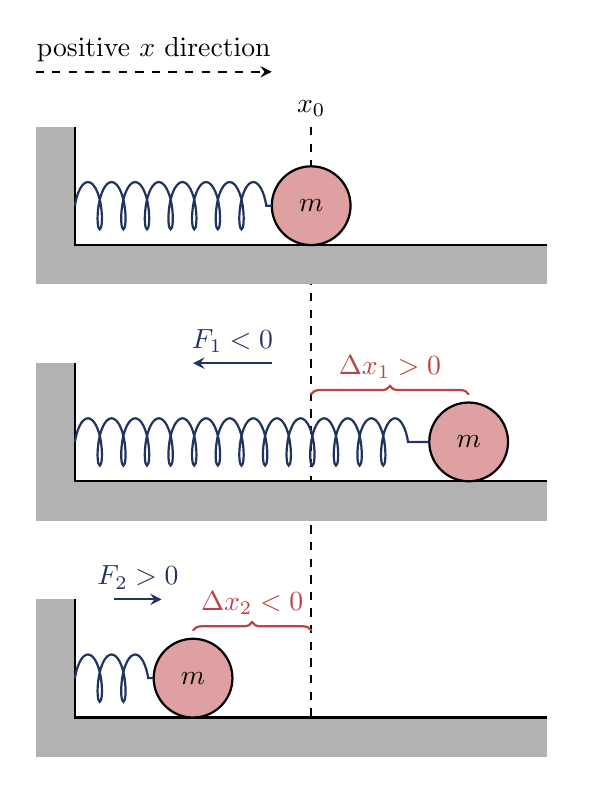
\begin{tikzpicture}
      \coordinate (x0) at (3,1.5);
      \draw[thick, dashed, black] (x0 |- 0,1) node [above] {$x_0$} -- ++(0,-8);
      \draw[thick, dashed,-stealth] (-0.5, 1.7) -- ++(3,0) node [midway, above] {positive $x$ direction};

      \draw[line width=5mm, black!30] (-0.25,1) -- ++(0,-1.75) -- ++(6.25,0);
      \draw[thick] (0,1) -- ++(0,-1.5) -- ++(6,0);
      \draw[thick, fill=xred!50] (3,0) circle (0.5) node (m1) {$m$};
      \draw[springcoil, xdarkblue] (0,0) -- ($(m1)-(0.5,0)$);

      \draw[line width=5mm, black!30] (-0.25,-2) -- ++(0,-1.75) -- ++(6.25,0);
      \draw[thick] (0,-2) -- ++(0,-1.5) -- ++(6,0);
      \draw[thick, fill=xred!50] (5,-3) circle (0.5) node (m2) {$m$};
      \draw[springcoil, xdarkblue] (0,-3) -- ($(m2)-(0.5,0)$);

      \draw[line width=5mm, black!30] (-0.25,-5) -- ++(0,-1.75) -- ++(6.25,0);
      \draw[thick] (0,-5) -- ++(0,-1.5) -- ++(6,0);
      \draw[thick, fill=xred!50] (1.5,-6) circle (0.5) node (m3) {$m$};
      \draw[springcoil, xdarkblue] (0,-6) -- ($(m3)-(0.5,0)$);

      \draw[xred, thick, cap=round, decorate, decoration={brace, amplitude=3pt, raise=3pt}] (m1 |- 0,-2.5) -- (m2 |- 0,-2.5) node[midway, above, yshift=5pt]{$\Delta x_{1}>0$};
      \draw[xred, thick, cap=round, decorate, decoration={brace, amplitude=3pt, raise=3pt, mirror}] (m1 |- 0,-5.5) -- (m3 |- 0,-5.5) node[midway, above, yshift=5pt]{$\Delta x_{2}<0$};

      \draw[-stealth, thick, xdarkblue] (2.5,-2) -- ++(-1,0) node[midway, above] {$F_{1}<0$};
      \draw[-stealth, thick, xdarkblue] (0.5,-5) -- ++(0.6,0) node[midway, above] {$F_{2}>0$};
    \end{tikzpicture}
  \end{center}
  \caption{A simple spring-mass system with spring constant $k$ and a mass $m$. The top figure shows the spring at rest - i.e. when the mass is located at position $x_{0}$ the spring applies no force on the mass (since $\Delta x = x_{m}-x_{0}=0$). The middle figure show the spring being at a \textit{positive} displacement $\Delta x_{1}>0$, causing the spring to pull back with a negative force $F_{1}=-k\Delta x_{1}$. The bottom picture shows the spring contracting by $\Delta x_{2}<0$, casing the spring to apply a positive force $F_{2}=-k\Delta x_{2}$ on the mass.}\label{fig:simple_spring}
\end{figure}


% \section{Simulating Simple Mechanics}
\subsection{Forward Euler Method}
\subsection{Backward Euler Method}
\subsection{Verlet Integration}
\subsection{Runge-Kutta Method}

% \input{waves}
\chapter{Thermodynamics}

\section{Preface}
Text text text

\section{Ideal gas}
\subsection{Theory}
There are several commonly used models for the behaviour of gasses. A very simple yet powerful one is the \textbf{ideal gas} model: it describes gas particles as being perfect spheres which move around in an enclosed container and undergo elastic collisions with other particles and the walls of the container. In common conditions such as atmospheric pressure and temperatures around $\SI{300}{\kelvin}$, gasses such as helium (\ce{He}), argon (\ce{Ar}), nitrogen (\ce{N2}), oxygen (\ce{O2}) and carbon dioxide (\ce{CO2}) behave like ideal gasses (assuming no chemical reations take place). However, the ideal gas model fails under high pressures, low temperatures, chemical interactions and some physical processes such as adsorption or multipolar interactions.

The principle equation describing an ideal gas is the \textbf{ideal gas law}:
\begin{equation}
	PV = nRT,
	\label{eq:ideal_gas_law}
\end{equation}
where (SI units in parentheses):
\begin{itemize}
	\item $P$ is the pressure of the gas ($\si{\pascal}$),
	\item $V$ is the volume of the container ($\si{\cubic\metre}$),
	\item $n$ is the amount of gas ($\si{\mol}$),
	\item $R$ is the \textbf{gas constant}, $R=\SI{8.314}{\joule\per\kelvin\per\mol}$, and
	\item $T$ is the temperature of the gas ($\si{\kelvin}$).
\end{itemize}

\subsubsection{Maxwell-Boltzman distribution}
\subsubsection{Mean free path}
\subsubsection{Temperature from energy}

\subsection{Simulating an ideal gas using perfectly elastic spheres}
Text text text

% subsubsection: sphere-wall collision
\subsubsection{Sphere-wall collision}
An elastic collision between a particle and a wall causes the particle's velocity to flip in the direction of the wall's normal (\autoref{fig:particle_wall_collision}).

\begin{figure}
	\begin{center}
		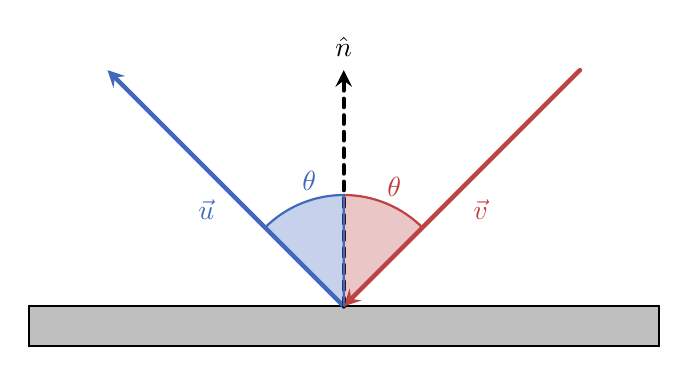
\begin{tikzpicture}
			\draw[thick, fill=black!25] (-4,-0.5) rectangle (4,0);
			\draw[vector={xred}]  (3,3) -- (0,0)  node [midway, below right] {$\vec{v}$};
			\draw[vector={xblue}] (0,0) -- (-3,3) node [midway, below left]  {$\vec{u}$};
			\draw[vector={black}, dashed] (0,0) -- (0,3) node [pos=1.1] {$\hat{n}$};
			\draw[filledangle={xred}] (0,0) -- (1,1) arc (45:90:{sqrt(2)}) node [above, pos=0.4] {$\theta$};
			\draw[filledangle={xblue}] (0,0) -- (0,{sqrt(2)}) arc (90:135:{sqrt(2)}) node [above, pos=0.4] {$\theta$};
		\end{tikzpicture}
	\end{center}
	\caption{Collision of a particle and a wall. The particle bounces in such a way that the component of its velocity $\vec{v}$ in the direction of the wall's normal $\hat{n}$ is flipped. The resulting velocity $\vec{u}$ has the same angle to $\hat{n}$ as $\vec{v}$ does.}
	\label{fig:particle_wall_collision}
\end{figure}

The component of $\vec{v}$ in the direction of $\hat{n}$ is
\begin{equation}
	\vec{v}_{\parallel} = \innerproduct{\vec{v}}{\hat{n}}\hat{n}.
	% \label{eq:label}
\end{equation}
Therefore, the component of $\vec{v}$ orthogonal to $\hat{n}$ is
\begin{equation}
	\vec{v}_{\perp} = \vec{v} - \vec{v}_{\parallel} = \vec{v} - \innerproduct{\vec{v}}{\hat{n}}\hat{n}.
	% \label{eq:label}
\end{equation}
In the case of $\vec{u}$, the orthogonal component is the same as that of $\vec{v}$, but the parallel component is inverted:
\begin{equation}
	\begin{aligned}
		\vec{u}_{\perp}     & = \vec{v}_{\perp},      \\
		\vec{u}_{\parallel} & = -\vec{v}_{\parallel}.
	\end{aligned}
	% \label{eq:label}
\end{equation}
and altogether we get
\begin{equation}
	\begin{aligned}
		\vec{u} & = \vec{u}_{\perp} + \vec{u}_{\parallel}                                                     \\
		        & = \vec{v} - \innerproduct{\vec{v}}{\hat{n}}\hat{n} - \innerproduct{\vec{v}}{\hat{n}}\hat{n} \\
		        & = \vec{v}-2\innerproduct{\vec{v}}{\hat{n}}\hat{n}.
	\end{aligned}
	\label{eq:elastic_sphere_wall_collision}
\end{equation}

\begin{example}{A simple sanity check}{}
	To make a simple validation of this equation, let's examine the case for a collision with a wall which is oriented in the $xy$-plane (i.e. its normal points in the $z$-direction): given the velocity $\vec{v}=\colvec{v_{x};v_{y};v_{z}}$, \autoref{eq:elastic_sphere_wall_collision} becomes
	\begin{align*}
		\vec{u} & = \vec{v}-2\innerproduct{\vec{v}}{\hat{n}}\hat{n}                                                     \\
		        & = \colvec{v_{x};v_{y};v_{z}}-2\innerproduct{\colvec{v_{x};v_{y};v_{z}}}{\colvec{0;0;1}}\colvec{0;0;1} \\
		        & = \colvec{v_{x};v_{y};v_{z}}-2(\cancel{v_{x}\cdot0}+\cancel{v_{y}\cdot0}+v_{z}\cdot1)\colvec{0;0;1}   \\
		        & = \colvec{v_{x};v_{y};v_{z}}-2v_{z}\colvec{0;0;1}                                                     \\
		        & = \colvec{v_{x};v_{y};v_{z}}-2\colvec{0;0;v_{z}}                                                      \\
		        & =  \colvec{v_{x};v_{y};v_{z}}+\colvec{0;0;-2v_{z}}                                                    \\
		        & =  \colvec{v_{x};v_{y};-v_{z}},
	\end{align*}
	as expected.
\end{example}

\begin{note}{Studying advice}{}
	The reader is encouraged to repeat the above calculation for the cases of walls oriented in the $xz$- and $yz$-planes.
\end{note}

\subsubsection{Sphere-sphere collision}
Consider two solid spheres which have a single point of contact $\bm{A}$. Let $m_{1}, r_{1}, \vec{x}_{1}$ and $\vec{v}_{1}$ be the mass, radius, position and velocity of the first sphere, and $m_{2}, r_{2}, \vec{x}_{2}$ and $\vec{v}_{2}$ the respective quantities for the second sphere (\autoref{fig:elastic_collision}). The line connecting the centers of the two spheres is in the direction $\hat{n}$ (without loss of generality let us assume that the normal vector $\hat{n}$ points from $\vec{x}_{1}$ towards $\vec{x}_{2}$). The unit vector $\hat{t}$ is orthogonal to $\hat{n}$ (and without loss of generality we will assume that it is oriented counter-clockwise from $\hat{n}$).

\begin{figure}
	\begin{center}
		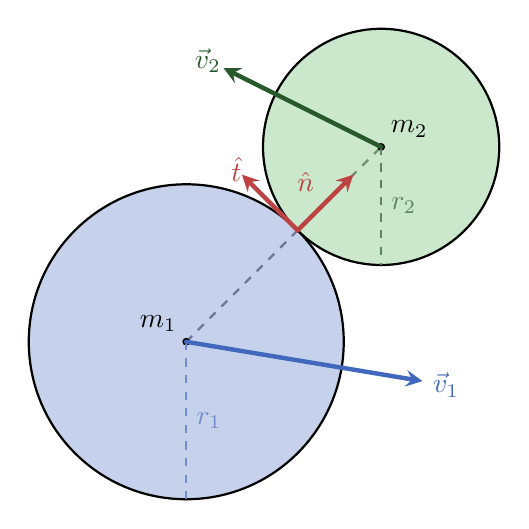
\begin{tikzpicture}
			\coordinate (xA) at (0, 0);
			\pgfmathsetmacro{\rA}{2}
			\pgfmathsetmacro{\rB}{1.5}
			\pgfmathsetmacro{\th}{45}
			\coordinate (xB) at ({(\rA+\rB)*cos(\th)},{(\rA+\rB)*sin(\th)});
			\coordinate (uAB) at ({\rA*cos(\th)},{\rA*sin(\th)});
			\draw[thick, dashed, black!50] (xA) -- (xB);

			\tikzset{
				sphere/.style={thick, fill=#1, fill opacity=0.3},
				radius/.style={thick, dashed, draw=#1},
			}
			\draw[sphere={xblue}]  (xA) circle (\rA);
			\draw[sphere={xgreen}] (xB) circle (\rB);
			\fill (xA) circle (0.05) node [above left]  {$m_{1}$};
			\fill (xB) circle (0.05) node [above right] {$m_{2}$};
			\draw[radius={xblue!75}] (xA) -- ++(0,-\rA) node [xblue!75, midway, right] {$r_{1}$};
			\draw[radius={xdarkgreen!75}] (xB) -- ++(0,-\rB) node [xdarkgreen!75, midway, right]  {$r_{2}$};

			\draw[vector={xblue}] (xA) -- ++(3,-0.5) node [pos=1.1] {$\vec{v}_{1}$};
			\draw[vector={xdarkgreen}] (xB) -- ++(-2,1.0) node [pos=1.1] {$\vec{v}_{2}$};

			\draw[vector={xred}] (uAB) -- ++({cos(\th)},{sin(\th)}) node [midway, above left] {$\hat{n}$};
			\draw[vector={xred}] (uAB) -- ++({cos(\th+90)},{sin(\th+90)}) node [pos=1.1] {$\hat{t}$};
		\end{tikzpicture}
	\end{center}
	\caption{Text text text}
	\label{fig:elastic_collision}
\end{figure}

Note that we did not define a coordinate system, nor the number of dimensions $d$ for the problem. The only restriction is that $d\geq2$.

Conservation of momentum means that the velocities of the spheres following the collision, $\vec{u}_{1},\vec{u}_2$, are related to their velocities before the collision by
\begin{equation}
	\begin{aligned}
		                 & m_{1}\vec{v}_{1} + m_{2}\vec{v}_{2} = m_{1}\vec{u}_{1} + m_{2}\vec{u}_{2}                   \\
		\Rightarrow\quad & m_{1}\left(\vec{v}_{1} - \vec{u}_{1}\right)  = m_{2}\left(\vec{u}_{2} - \vec{v}_{2}\right).
	\end{aligned}
	\label{eq:elastic_collision_coservation_of_momentum}
\end{equation}

Conservation of energy means that the velocities are also related by
\begin{equation}
	\begin{aligned}
		                 & \frac{1}{2}m_{1}\norm{\vec{v}_{1}}^{2} + \frac{1}{2}m_{2}\norm{\vec{v}_{2}}^{2} = \frac{1}{2}m_{1}\norm{\vec{u}_{1}}^{2} + \frac{1}{2}m_{2}\norm{\vec{u}_{2}}^{2} \\
		\Rightarrow\quad & m_{1}\left(\norm{\vec{v}_{1}}^{2} - \norm{\vec{u}_{1}}^{2}\right) = m_{2}\left(\norm{\vec{u}_{2}}^{2} - \norm{\vec{v}_{2}}^{2}\right).
	\end{aligned}
	\label{eq:elastic_collision_coservation_of_energy}
\end{equation}

However, the forces involved in the collision can not have a component in the $\hat{t}$ direction, and are limited to only point in the $\hat{n}$ direction. Therefore, we can reduce the problem to this direction only by projecting all velocities involved in the problem on $\hat{n}$, i.e. \autoref{eq:elastic_collision_coservation_of_momentum} becomes
\begin{equation}
	m_{1}\innerproduct{\vec{v}_{1}}{\hat{n}} + m_{2}\innerproduct{\vec{v}_{2}}{\hat{n}} = m_{1}\innerproduct{\vec{u}_{1}}{\hat{n}} + m_{2}\innerproduct{\vec{u}_{2}}{\hat{n}}.
	\label{eq:elastic_collision_coservation_of_momentum_projection}
\end{equation}

TEXT TEXT TEXT

\begin{equation}
	\begin{aligned}
		\vec{u}_{1} & = \vec{v}_{1} - \frac{2m_{2}}{m_{1}+m_{2}}\innerproduct{\vec{v}_{1}-\vec{v}_{2}}{\hat{n}}\hat{n}, \\
		\vec{u}_{2} & = \vec{v}_{2} + \frac{2m_{1}}{m_{1}+m_{2}}\innerproduct{\vec{v}_{1}-\vec{v}_{2}}{\hat{n}}\hat{n}.
	\end{aligned}
\end{equation}

To avoid reduntant calculations, we can factor out the common quantity of both velocities:
\begin{equation}
	K = \frac{2}{m_{1}+m_{2}}\innerproduct{\vec{v}_{1}-\vec{v}_{2}}{\hat{n}}\hat{n},
	\label{eq:elastic_collision_common_quantity}
\end{equation}
yielding
\begin{equation}
	\begin{aligned}
		\vec{u}_{1} & = \vec{v}_{1}-Km_{2}, \\
		\vec{u}_{2} & = \vec{v}_{2}+Km_{1}.
	\end{aligned}
	\label{eq:elastic_collision_final_equation}
\end{equation}

\subsubsection{Reducing collision test complexity}
% BBOX, Neighbor lists, etc.

\section{Brownian dynamics}

% \input{molecular_dynamics}
\makeatother

\end{document}
